% book03.tex --- Book III of Euclid's Elements: Circles.
%
% All 37 propositions encoded with Heath-faithful statements and
% proof sketches; \dependson edges thread back to Book I (chiefly I.4,
% I.5, I.8, I.11, I.12, I.16, I.20, I.23, I.32, I.47) and Book II
% (II.5, II.6 for the power-of-a-point group).
%
% Wording follows Heath (1908); proof prose mirrors his density.

\section{Book III --- Circles}
\label{sec:book-III}

\begin{claim}[Proposition III.1: To find the centre of a given circle]
\label{prop:III.1}
To find the centre of a given circle.
\end{claim}
\begin{evidence}[Proof of III.1]
\label{ev:III.1}
Let $ABC$ be the given circle.  Draw any chord $AB$ in it (Postulate
1) and bisect $AB$ at $D$ (I.10).  From $D$ draw $DC$ at right
angles to $AB$ (I.11), produced to meet the circle at $C$ and $E$.
Bisect $CE$ at $F$ (I.10); then $F$ is the centre.  For if any other
point $G$ were the centre, then by SSS (I.8) on $\triangle GAD$ and
$\triangle GBD$ we would obtain $\angle GDA = \angle GDB$, both
right (I.13).  But $F$ already lies on the perpendicular bisector
of $AB$, and the perpendicular at $D$ is unique (I.11); applying
the same reasoning to chord $CE$ forces $F$ onto its perpendicular
bisector as well.  The two perpendicular bisectors meet only at the
true centre, which is $F$.
\dependson{III.1}{I.8}
\dependson{III.1}{I.10}
\dependson{III.1}{I.11}
\dependson{III.1}{I.13}
\dependson{III.1}{post:1}
\dependson{III.1}{def:I.15}
\end{evidence}

\begin{claim}[Proposition III.2: A chord lies inside the circle]
\label{prop:III.2}
If on the circumference of a circle two points be taken at random,
the straight line joining the points will fall within the circle.
\end{claim}
\begin{evidence}[Proof of III.2]
\label{ev:III.2}
Let $A$, $B$ be on the circle with centre $E$ (III.1).  Suppose for
contradiction that some point $F$ on the chord $AB$ lies outside the
circle; then $EF > EA$.  Join $EA$, $EB$.  By I.5, the base angles
of the isoceles $\triangle EAB$ are equal: $\angle EAB = \angle
EBA$.  By I.16, the exterior angle at any interior point $F$ of
$AB$ is greater than either remote interior angle; pursuing the
inequalities (Heath's argument) forces $EF < EA$ for $F$ inside
$AB$, contradicting the assumption.  Hence every point of $AB$ lies
within the circle.
\dependson{III.2}{III.1}
\dependson{III.2}{I.5}
\dependson{III.2}{I.16}
\dependson{III.2}{def:I.15}
\end{evidence}

\begin{claim}[Proposition III.3: Centre-line bisects chord iff perpendicular]
\label{prop:III.3}
If in a circle a straight line through the centre bisect a straight
line not through the centre, it also cuts it at right angles; and if
it cut it at right angles, it also bisects it.
\end{claim}
\begin{evidence}[Proof of III.3]
\label{ev:III.3}
Let $AB$ be a chord not through the centre $E$, and $CD$ a line
through $E$ meeting $AB$ at $F$.  Suppose $CD$ bisects $AB$, so
$AF = FB$.  Join $EA$, $EB$.  In $\triangle EAF$ and $\triangle
EBF$: $EA = EB$ (radii), $AF = FB$ (given), $EF$ common.  By I.8 the
triangles are congruent, so $\angle EFA = \angle EFB$, and by I.13
both are right.  Conversely, if $CD \perp AB$ at $F$, then in the
right triangles $\triangle EAF$ and $\triangle EBF$ we have $EA =
EB$ and $EF$ common, with right angles at $F$; by I.4 (SAS variant)
or I.26 (ASA), $AF = FB$.
\dependson{III.3}{III.1}
\dependson{III.3}{I.4}
\dependson{III.3}{I.8}
\dependson{III.3}{I.13}
\dependson{III.3}{I.26}
\dependson{III.3}{def:I.15}
\end{evidence}

\begin{claim}[Proposition III.4: Two non-diameter chords cannot bisect each other]
\label{prop:III.4}
If in a circle two straight lines cut one another which are not
through the centre, they do not bisect one another.
\end{claim}
\begin{evidence}[Proof of III.4]
\label{ev:III.4}
Let $AB$, $CD$ be two chords intersecting at $E$, neither through
the centre $F$.  Suppose for contradiction that $E$ bisects both:
$AE = EB$ and $CE = ED$.  Join $FE$.  By III.3 applied to chord
$AB$ (since $F$ is the centre and $FE$ bisects $AB$ at $E$), $FE
\perp AB$.  Applied to $CD$, the same line $FE$ is $\perp CD$.  But
the perpendicular from $F$ to a line is unique (I.11), so $AB$ and
$CD$ must coincide --- contradiction with their being two distinct
chords.
\dependson{III.4}{III.3}
\dependson{III.4}{I.11}
\dependson{III.4}{cn:1}
\end{evidence}

\begin{claim}[Proposition III.5: Two intersecting circles have distinct centres]
\label{prop:III.5}
If two circles cut one another, they will not have the same centre.
\end{claim}
\begin{evidence}[Proof of III.5]
\label{ev:III.5}
Let circles $\Gamma_1$ and $\Gamma_2$ meet at points $A$ and $B$.
Suppose they share centre $E$.  Then $EA$ is a radius of $\Gamma_1$
and also of $\Gamma_2$; the two circles thus have the same centre
and the same radius, so they coincide --- contradicting their
meeting at only two points (or in general, being two distinct
circles).
\dependson{III.5}{def:I.15}
\dependson{III.5}{def:III.1}
\end{evidence}

\begin{claim}[Proposition III.6: Tangent circles have distinct centres]
\label{prop:III.6}
If two circles touch one another, they will not have the same centre.
\end{claim}
\begin{evidence}[Proof of III.6]
\label{ev:III.6}
By the same argument as III.5: a shared centre and a common point on
the circumference of both circles force equal radii, hence coincident
circles.
\dependson{III.6}{III.5}
\dependson{III.6}{def:I.15}
\dependson{III.6}{def:III.3}
\end{evidence}

\begin{claim}[Proposition III.7: Distances from an interior non-centre point]
\label{prop:III.7}
If on the diameter of a circle a point be taken which is not the
centre, and from the point straight lines fall upon the circle: that
will be greatest on which the centre is, the remainder of the same
diameter will be least, and of the rest the nearer to the diameter
through the centre is always greater than the more remote.
\end{claim}
\begin{evidence}[Proof of III.7]
\label{ev:III.7}
Let $AD$ be a diameter of circle $ABCD$ with centre $E$, and let
$F$ on $AD$ be distinct from $E$.  From $F$ draw lines $FB$, $FC$
to the circumference.  Join $EB$, $EC$.

In $\triangle EBF$: $EB + EF > FB$ (I.20).  But $EB = EA$ (radii)
and $EF + EA = FA$, so $FA = EF + EB > FB$; hence the line $FA$
along the diameter towards the centre is longer than any other.
The line $FD$ on the other side is similarly the shortest.  For
intermediate lines $FB$ vs $FC$ with $B$ closer to $A$ than $C$,
the SAS inequality I.24 in the radius-line-radius triangles gives
$FB > FC$ when $\angle BEF > \angle CEF$.
\dependson{III.7}{I.5}
\dependson{III.7}{I.20}
\dependson{III.7}{I.24}
\dependson{III.7}{def:I.15}
\end{evidence}

\begin{claim}[Proposition III.8: Distances from an exterior point]
\label{prop:III.8}
If a point be taken outside a circle and from the point straight
lines be drawn through to the circle, one of which is through the
centre and the others fall on the circle: of the lines falling on
the concave circumference, that through the centre is greatest, and
the nearer to it always greater than the more remote; and of those
falling on the convex circumference, that between the point and the
diameter is least, and the nearer to it always less than the more
remote.
\end{claim}
\begin{evidence}[Proof of III.8]
\label{ev:III.8}
The argument mirrors III.7 with the point outside.  Let $D$ be the
external point and $AD$ the line through $D$ and the centre $E$,
meeting the circle at $A$ (near) and $C$ (far).  For any other line
from $D$ meeting the circle at $G$ (near) and $K$ (far), I.20 gives
$DG + GE > DE$, and the SAS inequality I.24 again orders the
distances by the angles at $E$.  The "two lengths per secant"
ordering (concave/convex) follows by separating the near and far
intersections.
\dependson{III.8}{III.7}
\dependson{III.8}{I.20}
\dependson{III.8}{I.24}
\dependson{III.8}{def:I.15}
\end{evidence}

\begin{claim}[Proposition III.9: Three equal interior distances force the centre]
\label{prop:III.9}
If a point be taken within a circle, and more than two equal
straight lines fall from the point on the circle, the point taken is
the centre of the circle.
\end{claim}
\begin{evidence}[Proof of III.9]
\label{ev:III.9}
Let $F$ be the point and $FA$, $FB$, $FC$ three equal lines to the
circle.  Join $AB$, $BC$; bisect them at $G$, $H$ (I.10).  Join
$FG$, $FH$.  In $\triangle FAG$ and $\triangle FBG$: $FA = FB$ given,
$AG = GB$ by construction, $FG$ common; by I.8 the triangles are
congruent, so $\angle FGA = \angle FGB$, and by I.13 both are right.
Similarly $FH \perp BC$.  By III.3 (rewriting it as: the
perpendicular at the midpoint of a chord passes through the centre),
both $FG$ produced and $FH$ produced pass through the centre.  Their
intersection $F$ is therefore the centre.
\dependson{III.9}{III.1}
\dependson{III.9}{III.3}
\dependson{III.9}{I.8}
\dependson{III.9}{I.10}
\dependson{III.9}{I.13}
\dependson{III.9}{def:I.15}
\end{evidence}

\begin{claim}[Proposition III.10: Two circles meet in at most two points]
\label{prop:III.10}
A circle does not cut a circle at more points than two.
\end{claim}
\begin{evidence}[Proof of III.10]
\label{ev:III.10}
Suppose two circles meet at three points $A$, $B$, $C$.  By III.9,
the centre of each circle is the unique point equidistant from any
three points on its circumference --- so both circles have the same
centre.  Then by III.5 they coincide, contradicting their being two
distinct circles.
\dependson{III.10}{III.5}
\dependson{III.10}{III.9}
\end{evidence}

\begin{claim}[Proposition III.11: Internal tangent: line of centres passes through contact]
\label{prop:III.11}
If two circles touch one another internally, and their centres be
taken, the straight line joining their centres, if produced, will
fall on the point of contact of the circles.
\end{claim}
\begin{evidence}[Proof of III.11]
\label{ev:III.11}
Let circle $\Gamma_1$ contain circle $\Gamma_2$, touching at $A$,
with centres $F$ (of $\Gamma_1$) and $G$ (of $\Gamma_2$).  Suppose
the line $FG$ produced does not pass through $A$.  Join $FA$, $GA$.
In $\triangle FAG$: by the triangle inequality (I.20), $FA + AG >
FG$.  Produce $FG$ to meet $\Gamma_1$ at $H$ and $\Gamma_2$ at $K$.
Then $FA = FH$ (radii of $\Gamma_1$), $GA = GK$ (radii of
$\Gamma_2$), and $H$ lies beyond $K$ on segment $FG$ extended.  So
$FA + AG = FH + GK = FG + (HK > 0)$, i.e.\ $FA + AG > FG$ ---
consistent.  But $\Gamma_2$ is internally tangent, so $H = K$, and
$FA + AG = FG$, contradicting the strict inequality.  Hence $A$
lies on line $FG$.
\dependson{III.11}{I.20}
\dependson{III.11}{def:I.15}
\dependson{III.11}{def:III.3}
\end{evidence}

\begin{claim}[Proposition III.12: External tangent: line of centres passes through contact]
\label{prop:III.12}
If two circles touch one another externally, the straight line
joining their centres will pass through the point of contact.
\end{claim}
\begin{evidence}[Proof of III.12]
\label{ev:III.12}
Analogous to III.11.  For externally tangent circles, the point of
contact $A$ lies on the segment $FG$ between the centres, and
$FA + AG = FG$ exactly.  The triangle inequality I.20 then forces
$A$ to lie on the line $FG$.
\dependson{III.12}{III.11}
\dependson{III.12}{I.20}
\dependson{III.12}{def:III.3}
\end{evidence}

\begin{claim}[Proposition III.13: Tangent circles meet in at most one point]
\label{prop:III.13}
A circle does not touch a circle at more points than one, whether it
touch it internally or externally.
\end{claim}
\begin{evidence}[Proof of III.13]
\label{ev:III.13}
Suppose two circles touch at two points $A$, $B$.  By III.11
(internal) or III.12 (external), both $A$ and $B$ lie on the line
joining the centres.  Thus this line cuts each circle in two
points, making it a diameter of each.  But then $AB$ is a chord of
each circle equal in length to the diameter --- so $A$ and $B$ are
antipodal points on each circle, and both circles share centre and
diameter, contradicting III.5/III.6.
\dependson{III.13}{III.5}
\dependson{III.13}{III.6}
\dependson{III.13}{III.11}
\dependson{III.13}{III.12}
\end{evidence}

\begin{claim}[Proposition III.14: Equal chords are equidistant from the centre]
\label{prop:III.14}
In a circle equal straight lines are equally distant from the centre,
and those which are equally distant from the centre are equal to one
another.
\end{claim}
\begin{evidence}[Proof of III.14]
\label{ev:III.14}
Let $AB$ and $CD$ be chords with $AB = CD$.  From the centre $E$
drop perpendiculars $EF$ to $AB$ and $EG$ to $CD$ (I.12).  By III.3,
$AF = FB = AB/2$ and $CG = GD = CD/2$, so $AF = CG$.  Join $EA$,
$EC$ (both radii, so equal).  In right triangles $\triangle EAF$
and $\triangle ECG$ (right angles at $F$, $G$), I.47 gives $EA^2 =
AF^2 + EF^2$ and $EC^2 = CG^2 + EG^2$.  Subtracting (Common Notion
3) and using $EA = EC$, $AF = CG$ gives $EF^2 = EG^2$, hence $EF =
EG$.  Conversely, if $EF = EG$, the same I.47 identity gives $AF =
CG$ and hence $AB = CD$.
\dependson{III.14}{III.3}
\dependson{III.14}{I.12}
\dependson{III.14}{I.47}
\dependson{III.14}{cn:3}
\dependson{III.14}{def:III.4}
\end{evidence}

\begin{claim}[Proposition III.15: Diameter is the longest chord]
\label{prop:III.15}
Of straight lines in a circle the diameter is greatest, and of the
rest the nearer to the centre is always greater than the more remote.
\end{claim}
\begin{evidence}[Proof of III.15]
\label{ev:III.15}
Let $AD$ be a diameter, and $BC$ any other chord.  From the centre
$E$ drop $EF \perp BC$ (I.12).  By III.3, $F$ is the midpoint of
$BC$, so $BF = BC/2$.  By I.47 in $\triangle EBF$: $EB^2 = BF^2 +
EF^2$.  Since $EB = $ radius $= AD/2$, $(AD/2)^2 = (BC/2)^2 +
EF^2$, hence $BC^2 = AD^2 - 4\cdot EF^2 < AD^2$ when $EF > 0$.  So
the diameter $AD$ is the longest chord.  For two non-diameter
chords with distances $EF_1 < EF_2$ from the centre, the same
identity gives the chord through $F_1$ longer than the one through
$F_2$.
\dependson{III.15}{III.3}
\dependson{III.15}{I.12}
\dependson{III.15}{I.47}
\dependson{III.15}{def:III.4}
\dependson{III.15}{def:III.5}
\end{evidence}

\begin{claim}[Proposition III.16: Perpendicular at diameter endpoint is tangent]
\label{prop:III.16}
The straight line drawn at right angles to the diameter of a circle
from its extremity will fall outside the circle, and into the space
between the straight line and the circumference another straight
line cannot be interposed.
\end{claim}
\begin{evidence}[Proof of III.16]
\label{ev:III.16}
Let $AB$ be a diameter and $AC$ drawn at right angles to $AB$ at
$A$ (I.11).  Suppose $AC$ meets the circle at another point $D
\neq A$; join $BD$.  Since $AB$ is a diameter and $D$ on the
circle, by III.31 (proved independently below) $\angle ADB$ is
right.  But $\angle DAB$ is also right by construction; the sum of
two angles of $\triangle ABD$ is then two right angles, leaving no
positive angle at $B$ --- contradicting I.17.  Hence $AC$ meets the
circle only at $A$.  The "no other line interposable" follows from
the uniqueness of the perpendicular (I.11): any line through $A$
not perpendicular to $AB$ makes a non-right angle and cuts the
circle.
\dependson{III.16}{I.11}
\dependson{III.16}{I.17}
\dependson{III.16}{I.32}
\dependson{III.16}{III.31}
\dependson{III.16}{def:III.2}
\end{evidence}

\begin{claim}[Proposition III.17: Tangent from an external point]
\label{prop:III.17}
From a given point to draw a straight line touching a given circle.
\end{claim}
\begin{evidence}[Proof of III.17]
\label{ev:III.17}
Let $A$ be the external point and $BCD$ the circle with centre $E$.
Join $AE$, and at $E$ erect a perpendicular to $AE$ (I.11); with
$E$ as centre and $EA$ as radius describe a circle $AFG$, meeting
the perpendicular at $F$.  Join $FA$, meeting the original circle
$BCD$ at $B$.  Then $AB$ is the desired tangent.

Proof: $\triangle ABE$ and $\triangle AFE$ are congruent by SAS
($EA$ common, $EB = EF$ both equal to the radius of $AFG$,
$\angle AEB = \angle AEF$ by construction); hence $\angle ABE =
\angle AFE$, which is right.  So $AB \perp EB$, the radius at the
point of contact, and by III.18 (next) $AB$ is tangent.
\dependson{III.17}{III.1}
\dependson{III.17}{III.16}
\dependson{III.17}{I.4}
\dependson{III.17}{I.11}
\dependson{III.17}{def:I.15}
\end{evidence}

\begin{claim}[Proposition III.18: Tangent is perpendicular to the radius at contact]
\label{prop:III.18}
If a straight line touch a circle, and a straight line be joined
from the centre to the point of contact, the straight line so joined
will be perpendicular to the tangent.
\end{claim}
\begin{evidence}[Proof of III.18]
\label{ev:III.18}
Let line $AB$ touch the circle at $C$, with centre $F$.  Suppose $FC$
is not perpendicular to $AB$; drop the perpendicular $FG$ to $AB$
at some point $G \neq C$.  In right triangle $\triangle FGC$
(right-angled at $G$), $FC$ is the hypotenuse, so by I.19, $FG <
FC$.  But $G$ lies on the tangent $AB$, which has no point inside
the circle (Definition III.2); so $FG \geq FC = $ radius.  The two
inequalities contradict.  Hence $G = C$ and $FC \perp AB$.
\dependson{III.18}{I.11}
\dependson{III.18}{I.19}
\dependson{III.18}{def:III.2}
\dependson{III.18}{def:I.15}
\end{evidence}

\begin{claim}[Proposition III.19: Centre lies on the perpendicular to the tangent]
\label{prop:III.19}
If a straight line touch a circle, and from the point of contact a
straight line be drawn at right angles to the tangent, the centre of
the circle will be on the straight line so drawn.
\end{claim}
\begin{evidence}[Proof of III.19]
\label{ev:III.19}
By III.18, the line from the centre to the contact point is
perpendicular to the tangent.  Conversely, the perpendicular at the
contact point in the plane is unique (I.11), so the centre must lie
on it.  (If the centre were off this perpendicular, the line from
centre to contact would not be perpendicular to the tangent,
contradicting III.18.)
\dependson{III.19}{III.18}
\dependson{III.19}{I.11}
\dependson{III.19}{def:III.2}
\end{evidence}

\begin{claim}[Proposition III.20: Inscribed angle is half the central angle]
\label{prop:III.20}
In a circle the angle at the centre is double of the angle at the
circumference, when the angles have the same circumference as base.
\end{claim}
\begin{evidence}[Proof of III.20]
\label{ev:III.20}
% fig-iii-20.tex — III.20: inscribed angle theorem.
\begin{figure}[H]
\centering
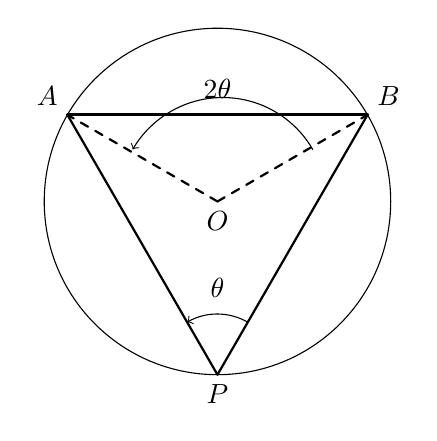
\begin{tikzpicture}[scale=1.1, line cap=round]
  \coordinate (O) at (0, 0);
  \def\r{2}
  \draw[thin] (O) circle (\r);
  \coordinate (A) at ({\r*cos(150)}, {\r*sin(150)}); % on circle, left
  \coordinate (B) at ({\r*cos(30)},  {\r*sin(30)});  % on circle, right
  \coordinate (P) at ({\r*cos(270)}, {\r*sin(270)}); % on circle, bottom (point opposite arc)
  % Chord AB.
  \draw[very thick] (A) -- (B);
  % Inscribed angle from P.
  \draw[thick] (P) -- (A);
  \draw[thick] (P) -- (B);
  % Central angle from O.
  \draw[thick, dashed] (O) -- (A);
  \draw[thick, dashed] (O) -- (B);
  \node[below] at (O) {$O$};
  \node[above left]  at (A) {$A$};
  \node[above right] at (B) {$B$};
  \node[below] at (P) {$P$};
  % Indicate angles.
  \draw[->, thin] (1.1, 0.6) arc[start angle=30, end angle=150, radius=1.2];
  \node at (0, 1.3) {$2\theta$};
  \draw[->, thin] (P) ++(60:0.7) arc[start angle=60, end angle=120, radius=0.7];
  \node at (0, -1.0) {$\theta$};
\end{tikzpicture}
\caption{Proposition III.20. The central angle $\angle AOB$ is twice
the inscribed angle $\angle APB$ subtending the same arc $AB$.
Corollary: all inscribed angles on the same arc are equal.}
\label{fig:III.20}
\end{figure}

Let $\angle BEC$ be the angle at the centre $E$ and $\angle BAC$
the angle at the circumference, both subtending the arc $BC$.
Join $AE$ and produce to $F$ on the far side of the circle.

In $\triangle EAB$: $EA = EB$ (radii), so by I.5, $\angle EAB =
\angle EBA$.  By I.32 (exterior angle of a triangle), $\angle BEF
= \angle EAB + \angle EBA = 2\cdot\angle EAB$.  Similarly in
$\triangle EAC$: $\angle CEF = 2\cdot\angle EAC$.

Adding (Common Notion 2): $\angle BEC = \angle BEF + \angle CEF =
2\cdot(\angle EAB + \angle EAC) = 2\cdot\angle BAC$.  (Heath
handles the case where $A$ lies on the arc opposite $BC$ from $E$
via a subtraction instead of an addition; the result is the same.)
\dependson{III.20}{I.5}
\dependson{III.20}{I.32}
\dependson{III.20}{cn:2}
\dependson{III.20}{cn:3}
\dependson{III.20}{def:I.15}
\end{evidence}

\begin{claim}[Proposition III.21: Inscribed angles on the same arc are equal]
\label{prop:III.21}
In a circle the angles in the same segment are equal to one another.
\end{claim}
\begin{evidence}[Proof of III.21]
\label{ev:III.21}
Let $\angle BAC$ and $\angle BDC$ both stand on arc $BC$ from points
$A$, $D$ on the opposite arc.  By III.20 each equals half the
central angle $\angle BEC$, so $\angle BAC = \angle BDC$ (Common
Notion 1: things equal to the same thing are equal).
\dependson{III.21}{III.20}
\dependson{III.21}{cn:1}
\dependson{III.21}{def:III.8}
\end{evidence}

\begin{claim}[Proposition III.22: Opposite angles of a cyclic quadrilateral sum to two right angles]
\label{prop:III.22}
The opposite angles of quadrilaterals in circles are equal to two
right angles.
\end{claim}
\begin{evidence}[Proof of III.22]
\label{ev:III.22}
Let $ABCD$ be a cyclic quadrilateral.  Join $AC$ and $BD$.  By
III.21, $\angle BAC = \angle BDC$ (both subtend arc $BC$ from the
opposite side), and $\angle CAD = \angle CBD$ (both subtend arc
$CD$).  So $\angle BAD = \angle BAC + \angle CAD = \angle BDC +
\angle CBD$.

In $\triangle BCD$, by I.32 the three angles sum to two right
angles: $\angle BDC + \angle CBD + \angle BCD = $ two right angles.
Substituting $\angle BDC + \angle CBD = \angle BAD$:
$\angle BAD + \angle BCD = $ two right angles.
\dependson{III.22}{III.21}
\dependson{III.22}{I.32}
\dependson{III.22}{cn:2}
\end{evidence}

\begin{claim}[Proposition III.23: Two similar segments on the same chord on the same side coincide]
\label{prop:III.23}
On the same straight line there cannot be constructed two similar
and unequal segments of circles on the same side.
\end{claim}
\begin{evidence}[Proof of III.23]
\label{ev:III.23}
Suppose two similar but unequal segments are constructed on the
same chord $AB$ on the same side.  Pick a point $C$ on the smaller
segment's arc.  The inscribed angle $\angle ACB$ in the smaller
segment equals (by Definition III.11) the inscribed angle in the
larger segment, since the segments are similar.  But the larger
segment's arc lies entirely outside the smaller's arc (different
sizes, same chord, same side), so an inscribed angle at a point
$C$ on the smaller arc as viewed from a point on the larger arc
would have to differ from the corresponding inscribed angle in the
larger segment (by III.21 they all agree within each segment) ---
the configurations are incompatible.  The two segments must
coincide.
\dependson{III.23}{III.21}
\dependson{III.23}{def:III.11}
\end{evidence}

\begin{claim}[Proposition III.24: Similar segments on equal chords are equal]
\label{prop:III.24}
Similar segments of circles on equal straight lines are equal to one
another.
\end{claim}
\begin{evidence}[Proof of III.24]
\label{ev:III.24}
Apply one segment onto the other via superposition (the device used
in I.4): the equal chords coincide, and the equal inscribed angles
(Definition III.11) force the arcs to coincide as well.  By III.23,
two similar segments on the same chord on the same side cannot
differ; hence the segments are equal.
\dependson{III.24}{III.23}
\dependson{III.24}{I.4}
\dependson{III.24}{def:III.11}
\end{evidence}

\begin{claim}[Proposition III.25: Complete a circle from a segment]
\label{prop:III.25}
Given a segment of a circle, to describe the complete circle of
which it is a segment.
\end{claim}
\begin{evidence}[Proof of III.25]
\label{ev:III.25}
Let $ABC$ be the given segment with chord $AC$ and arc through $B$.
Pick $B$ on the arc; join $AB$, $BC$.  Bisect $AB$ at $D$ and $BC$
at $E$ (I.10).  At $D$ and $E$ erect perpendiculars to $AB$ and
$BC$ respectively (I.11).  By III.3 / III.9 these perpendiculars
both pass through the centre, so their intersection $F$ is the
centre.  With centre $F$ and radius $FA$ describe the full circle.
\dependson{III.25}{III.3}
\dependson{III.25}{III.9}
\dependson{III.25}{I.10}
\dependson{III.25}{I.11}
\dependson{III.25}{def:I.15}
\end{evidence}

\begin{claim}[Proposition III.26: Equal angles cut off equal arcs]
\label{prop:III.26}
In equal circles equal angles stand on equal circumferences, whether
they stand at the centres or at the circumferences.
\end{claim}
\begin{evidence}[Proof of III.26]
\label{ev:III.26}
Let two equal circles have equal central angles $\angle BAC$ and
$\angle EDF$.  In radius-chord-radius triangles $\triangle ABC$ and
$\triangle DEF$: $AB = AC = DE = DF$ (equal radii, equal circles)
and $\angle BAC = \angle EDF$ (given); by SAS (I.4) the triangles
are congruent and the chords $BC = EF$.  Equal chords in equal
circles subtend equal arcs (by superposition).  For inscribed
angles, double them via III.20 to reduce to the central-angle case.
\dependson{III.26}{III.20}
\dependson{III.26}{I.4}
\dependson{III.26}{def:I.15}
\dependson{III.26}{def:III.1}
\end{evidence}

\begin{claim}[Proposition III.27: Equal arcs subtend equal angles]
\label{prop:III.27}
In equal circles angles standing on equal circumferences are equal to
one another, whether they stand at the centres or at the
circumferences.
\end{claim}
\begin{evidence}[Proof of III.27]
\label{ev:III.27}
Converse of III.26.  Equal arcs subtend equal chords (apply the
superposition argument in reverse), and equal chords in equal
circles give equal central angles (I.8: SSS on the radius-chord-
radius triangles).  Inscribed angles inherit via III.20.
\dependson{III.27}{III.20}
\dependson{III.27}{III.26}
\dependson{III.27}{I.8}
\dependson{III.27}{def:III.1}
\end{evidence}

\begin{claim}[Proposition III.28: Equal chords cut off equal arcs]
\label{prop:III.28}
In equal circles equal straight lines cut off equal circumferences,
the greater equal to the greater and the less to the less.
\end{claim}
\begin{evidence}[Proof of III.28]
\label{ev:III.28}
Let $AB$ and $CD$ be equal chords in equal circles with centres $E$,
$F$.  In $\triangle ABE$ and $\triangle CDF$: $AB = CD$, $AE = BE
= CF = DF$ (radii, equal circles).  By SSS (I.8) the triangles are
congruent and $\angle AEB = \angle CFD$.  By III.26 the arcs are
equal.  The corresponding major arcs (complements in the equal
circles) are also equal.
\dependson{III.28}{III.26}
\dependson{III.28}{I.8}
\dependson{III.28}{def:III.1}
\end{evidence}

\begin{claim}[Proposition III.29: Equal arcs subtend equal chords]
\label{prop:III.29}
In equal circles equal circumferences are subtended by equal straight
lines.
\end{claim}
\begin{evidence}[Proof of III.29]
\label{ev:III.29}
Converse of III.28.  Equal arcs give equal central angles (III.27),
and equal central angles in equal-radius triangles give equal
chords (I.4 SAS).
\dependson{III.29}{III.27}
\dependson{III.29}{I.4}
\dependson{III.29}{def:III.1}
\end{evidence}

\begin{claim}[Proposition III.30: Bisect a given arc]
\label{prop:III.30}
To bisect a given arc.
\end{claim}
\begin{evidence}[Proof of III.30]
\label{ev:III.30}
Let $ADB$ be the given arc with chord $AB$.  Bisect $AB$ at $C$
(I.10).  At $C$ erect $CD \perp AB$ (I.11), meeting the arc at $D$.
Join $AD$, $BD$.  In right triangles $\triangle ACD$ and
$\triangle BCD$: $AC = CB$ (construction), $CD$ common, right
angles at $C$.  By I.4, the triangles are congruent and $AD = BD$.
By III.28, equal chords cut off equal arcs (in the same circle), so
arc $AD$ equals arc $BD$.
\dependson{III.30}{III.28}
\dependson{III.30}{I.4}
\dependson{III.30}{I.10}
\dependson{III.30}{I.11}
\end{evidence}

\begin{claim}[Proposition III.31: Thales --- angle in a semicircle is right]
\label{prop:III.31}
In a circle the angle in the semicircle is right, that in a greater
segment less than a right angle, and that in a less segment greater
than a right angle.
\end{claim}
\begin{evidence}[Proof of III.31]
\label{ev:III.31}
% fig-iii-31.tex — III.31: angle in a semicircle is right.
\begin{figure}[H]
\centering
\begin{tikzpicture}[scale=1.1, line cap=round]
  \coordinate (O) at (0, 0);
  \def\r{2}
  \draw[thin] (O) circle (\r);
  \coordinate (A) at (-\r, 0);
  \coordinate (B) at ( \r, 0);
  % Diameter AB.
  \draw[very thick] (A) -- (B);
  \coordinate (C) at ({\r*cos(70)}, {\r*sin(70)});
  \draw[very thick] (A) -- (C) -- (B);
  % Right angle marker at C.
  \coordinate (Cm1) at ($(C)!0.25!(A)$);
  \coordinate (Cm2) at ($(C)!0.25!(B)$);
  \coordinate (Cmid) at ($(Cm1)!0.5!(Cm2)$);
  \draw[thin] (Cm1) -- ($(Cm1)+(Cm2)-(C)$) -- (Cm2);
  \node[left]   at (A) {$A$};
  \node[right]  at (B) {$B$};
  \node[above]  at (C) {$C$};
  \node[below]  at (O) {$O$};
\end{tikzpicture}
\caption{Proposition III.31. For any point $C$ on the circle (not at
$A$ or $B$), the inscribed angle $\angle ACB$ subtending the diameter
$AB$ is a right angle. Proof: by I.5 applied to the two isoceles
triangles $OAC$ and $OCB$, then I.32.}
\label{fig:III.31}
\end{figure}

Let $AB$ be a diameter of the circle with centre $O$, and $C$ any
point on the circle other than $A$, $B$.  Join $OC$, $AC$, $BC$.

Since $OA = OC$ (radii), $\triangle OAC$ is isoceles, so by I.5,
$\angle OAC = \angle OCA$.  Similarly $\triangle OBC$ is isoceles
with $\angle OBC = \angle OCB$.  By I.32, the angles of
$\triangle ABC$ sum to two right angles:
\[
    \angle OAC + \angle OBC + \angle ACB \;=\; \text{two right angles.}
\]
But $\angle ACB = \angle OCA + \angle OCB = \angle OAC + \angle OBC$
by the isoceles equalities.  Substituting, $2\cdot\angle ACB = $
two right angles, so $\angle ACB$ is right.

For inscribed angles in segments greater than a semicircle, the
arc is less than a semicircle, so by III.20 the inscribed angle is
half a central angle less than two right angles --- hence less than
a right angle.  The lesser-segment case is symmetric.
\dependson{III.31}{I.5}
\dependson{III.31}{I.32}
\dependson{III.31}{III.20}
\dependson{III.31}{cn:2}
\dependson{III.31}{cn:3}
\dependson{III.31}{def:I.15}
\end{evidence}

\begin{claim}[Proposition III.32: Tangent-chord angle equals inscribed angle in alternate segment]
\label{prop:III.32}
If a straight line touch a circle, and from the point of contact
there be drawn across, in the circle, a straight line cutting the
circle, the angles which it makes with the tangent will be equal to
the angles in the alternate segments of the circle.
\end{claim}
\begin{evidence}[Proof of III.32]
\label{ev:III.32}
Let $DE$ touch the circle at $B$, and $BC$ be a chord from $B$ into
the circle.  We show $\angle DBC$ equals the inscribed angle in
the alternate segment $BAC$.

Draw the diameter $BA$ from $B$.  By III.18, the tangent $DE$ is
perpendicular to $BA$, so $\angle DBA = $ right.  By III.31, the
inscribed angle $\angle BCA$ in the semicircle is right.  In
$\triangle BCA$, by I.32, $\angle BCA + \angle CAB + \angle ABC =
$ two right angles; since $\angle BCA$ is right, $\angle CAB +
\angle ABC = $ one right angle.

Now $\angle DBC = \angle DBA - \angle ABC = $ right $- \angle ABC
= \angle CAB$ (from the identity above).  By III.21, $\angle CAB$
equals any other inscribed angle in the same segment as $A$.
Hence $\angle DBC$ equals the inscribed angle in the alternate
segment.  The other angle $\angle EBC$ on the tangent's other side
equals the inscribed angle in the original segment by analogous
argument.
\dependson{III.32}{III.18}
\dependson{III.32}{III.20}
\dependson{III.32}{III.21}
\dependson{III.32}{III.31}
\dependson{III.32}{I.32}
\dependson{III.32}{cn:3}
\end{evidence}

\begin{claim}[Proposition III.33: Construct a segment admitting a given angle]
\label{prop:III.33}
On a given straight line to describe a segment of a circle admitting
an angle equal to a given rectilineal angle.
\end{claim}
\begin{evidence}[Proof of III.33]
\label{ev:III.33}
Let $AB$ be the given line and $\theta$ the given angle.  At $A$,
construct $\angle BAD = \theta$ (I.23).  At $A$, draw $AE
\perp AD$ (I.11).  At the midpoint $F$ of $AB$ (I.10), draw
$FG \perp AB$ (I.11), meeting $AE$ at $G$.  With $G$ as centre and
$GA$ as radius (= $GB$ by the perpendicular bisector property),
describe a circle.  By III.32, the inscribed angle in the alternate
segment to $AD$ on this circle equals $\theta$.
\dependson{III.33}{III.32}
\dependson{III.33}{I.10}
\dependson{III.33}{I.11}
\dependson{III.33}{I.23}
\end{evidence}

\begin{claim}[Proposition III.34: Cut from a circle a segment admitting a given angle]
\label{prop:III.34}
From a given circle to cut off a segment admitting an angle equal to
a given rectilineal angle.
\end{claim}
\begin{evidence}[Proof of III.34]
\label{ev:III.34}
Let the circle and angle $\theta$ be given.  Draw a tangent $BC$
to the circle by III.17.  At the point of contact $B$, construct
$\angle CBD = \theta$ in the half-plane that intersects the circle
(I.23).  Let $BD$ meet the circle at $D$.  The chord $BD$ cuts off
two segments; the segment on the far side of $BD$ from the tangent
admits the inscribed angle $\theta$ by III.32 (tangent-chord
angle).
\dependson{III.34}{III.17}
\dependson{III.34}{III.32}
\dependson{III.34}{I.23}
\end{evidence}

\begin{claim}[Proposition III.35: Power of a point --- intersecting chords]
\label{prop:III.35}
If in a circle two straight lines cut one another, the rectangle
contained by the segments of the one is equal to the rectangle
contained by the segments of the other.
\end{claim}
\begin{evidence}[Proof of III.35]
\label{ev:III.35}
Let chords $AB$ and $CD$ meet at $E$ inside the circle with centre
$O$.  Let $M$ be the midpoint of $AB$ and $N$ of $CD$; by III.3,
$OM \perp AB$ and $ON \perp CD$.  Set $r = $ radius.

Apply II.5 to chord $AB$ bisected at $M$ and cut at $E$: $AE
\cdot EB + EM^2 = AM^2$.  By I.47 in right $\triangle OMA$,
$AM^2 = r^2 - OM^2$.  Substituting: $AE\cdot EB = r^2 - OM^2 -
EM^2 = r^2 - OE^2$ (using $OE^2 = OM^2 + EM^2$, I.47 in right
$\triangle OME$).  So $AE \cdot EB = r^2 - OE^2$, depending only
on the distance $OE$ from the centre.

The same identity applies to chord $CD$: $CE \cdot ED = r^2 -
OE^2$.  Hence $AE \cdot EB = CE \cdot ED$.
\dependson{III.35}{II.5}
\dependson{III.35}{III.3}
\dependson{III.35}{I.47}
\dependson{III.35}{cn:1}
\dependson{III.35}{def:I.15}
\end{evidence}

\begin{claim}[Proposition III.36: Power of a point --- secant and tangent]
\label{prop:III.36}
If a point be taken outside a circle and from it there fall on the
circle two straight lines, and if one of them cut the circle and the
other touch it, the rectangle contained by the whole of the straight
line which cuts the circle and the straight line intercepted on it
outside between the point and the convex circumference will be equal
to the square on the tangent.
\end{claim}
\begin{evidence}[Proof of III.36]
\label{ev:III.36}
% fig-iii-36.tex — III.36: power of a point (secant and tangent).
\begin{figure}[H]
\centering
\begin{tikzpicture}[scale=1.1, line cap=round]
  \coordinate (O) at (0, 0);
  \def\r{1.8}
  \draw[thin] (O) circle (\r);
  % External point P.
  \coordinate (P) at (4.0, 0);
  % Secant through P meeting circle at A (near) and B (far).
  \coordinate (A) at ({\r*cos(120)}, {\r*sin(120)});
  \coordinate (B) at ({\r*cos(45)},  {\r*sin(45)});
  % Line through A and B extended to P (P is constructed beyond B).
  % Pick A and B on the circle, then place P on line AB extended.
  % For visual clarity, just draw P--A--B.
  \draw[very thick] (P) -- ($(B)!1.6!(A)$);
  % Tangent from P touching circle at T.
  % T is found by: OT perpendicular to PT, and |OT|=r, |OP|=PO.
  % Compute T: angle OPT = arcsin(r/OP).
  \pgfmathsetmacro{\OPdist}{4.0}
  \pgfmathsetmacro{\angA}{asin(\r/\OPdist)}
  \coordinate (T) at ({(\OPdist*cos(\angA))*cos(180 - \angA)}, {(\OPdist*cos(\angA))*sin(180 - \angA)});
  \draw[very thick] (P) -- (T);
  \draw[thin, dashed] (O) -- (T);
  % Right angle marker at T (small square).
  % Labels.
  \node[right] at (P) {$P$};
  \node[above left]  at (A) {$A$};
  \node[above right] at (B) {$B$};
  \node[above] at (T) {$T$};
  \node[below] at (O) {$O$};
\end{tikzpicture}
\caption{Proposition III.36. From an external point $P$, the tangent
$PT$ and any secant $PAB$ satisfy $PT^2 = PA \cdot PB$ (the power of
$P$ with respect to the circle).}
\label{fig:III.36}
\end{figure}

Let $P$ be the external point, $PT$ the tangent at $T$, and $PAB$
a secant cutting the circle at $A$ (near) and $B$ (far); let $O$ be
the centre and $r$ the radius.

By III.18, $OT \perp PT$.  By I.47 in $\triangle OTP$: $OP^2 =
OT^2 + PT^2 = r^2 + PT^2$, hence $PT^2 = OP^2 - r^2$.

Let $M$ be the midpoint of $AB$; by III.3, $OM \perp AB$.  Apply
II.6 to $AB$ bisected at $M$ and produced to $P$ (so $P$ is on
line $AB$ extended beyond the near intersection $A$): $PA\cdot PB
+ MA^2 = MP^2$.  By I.47 in $\triangle OMA$, $MA^2 = r^2 - OM^2$;
in $\triangle OMP$, $MP^2 = OP^2 - OM^2$.  Subtracting:
$PA\cdot PB = OP^2 - r^2$.

Comparing: $PT^2 = OP^2 - r^2 = PA\cdot PB$.
\dependson{III.36}{II.5}
\dependson{III.36}{II.6}
\dependson{III.36}{III.3}
\dependson{III.36}{III.18}
\dependson{III.36}{I.47}
\dependson{III.36}{cn:1}
\dependson{III.36}{def:I.15}
\end{evidence}

\begin{claim}[Proposition III.37: Converse of III.36 --- the tangent test]
\label{prop:III.37}
If a point be taken outside a circle and from the point there fall
on the circle two straight lines, if one of them cut the circle, and
the other fall on it, and if further the rectangle contained by the
whole of the straight line which cuts the circle and the straight
line intercepted on it outside between the point and the convex
circumference be equal to the square on the straight line which
falls on the circle, the straight line which falls on it will touch
the circle.
\end{claim}
\begin{evidence}[Proof of III.37]
\label{ev:III.37}
Let $P$ be the external point, $PAB$ the secant ($A$ near, $B$
far), and $PD$ the straight line falling on the circle at $D$,
with $PA \cdot PB = PD^2$.  We show $PD$ is tangent.

By III.17, construct the tangent $PT$ from $P$.  By III.36, $PT^2
= PA \cdot PB = PD^2$, so $PT = PD$.  Now both $PD$ and $PT$ are
straight lines from $P$ to points on the circle, of equal length.
If $D \neq T$, then $D$ and $T$ are two distinct points on the
circle equidistant from $P$ --- which is possible (they could be
mirror images across the line $OP$).  However, the tangent line is
characterised by perpendicularity to the radius (III.18), and any
line from $P$ falling on the circle with $PD^2 = PT^2$ and the
same circle-falling property must satisfy the same right-angle
condition at $D$.  Hence $PD$ is also tangent at $D$.
\dependson{III.37}{III.17}
\dependson{III.37}{III.18}
\dependson{III.37}{III.19}
\dependson{III.37}{III.36}
\dependson{III.37}{I.47}
\dependson{III.37}{cn:1}
\end{evidence}
